\documentclass[a4paper, 11pt]{exam}
\usepackage[T1]{fontenc}
\usepackage{titling}
\usepackage{url}
\usepackage{amsmath,amsthm,amssymb}
\usepackage{graphicx}
\usepackage{graphics}
\usepackage{listings}
\usepackage[dvipsnames]{xcolor}
\usepackage{tabularx}
\usepackage{ragged2e}
\usepackage{courier}
\usepackage{textcomp}
\usepackage{circuitikz}
\usepackage{tikz}
\usepackage{enumitem}
\usepackage{karnaugh-map}
\usepackage{bytefield}
\usepackage{mathrsfs}
\usepackage{cancel}
\usepackage[linesnumbered,ruled,vlined]{algorithm2e}
\usepackage{hyperref}
\newcommand{\invlaplace}[1]{%
\mathscr{L}^{-1}\left\{#1\right\}
}
\usepackage{tikz}
\usetikzlibrary{patterns}
\newcommand{\plotROC}[3]{
    % Draw the axes
    \draw[->] (-2.5,0) -- (2.5,0) node[anchor=north, xshift=.5cm, yshift=.3cm] {\( \text{Re}(z) \)};
    \draw[->] (0,-2.5) -- (0,2.5) node[anchor=east , xshift=.5cm, yshift=.2cm] {\( \text{Im}(z) \)};
    
    % Draw the Legend
    \draw (2.5,2.5) rectangle (4,1.5);
    \fill[red] (2.8,1.7) circle [radius=.05];
    \node[anchor=west] at (2.9, 1.7) {Poles};
    \fill[black] (2.8,2.2) circle [radius=.05];
    \node[anchor=west] at (2.9, 2.2) {Zeros};

    % Draw the circle with radius passed in
    \draw[dashed] (0,0) circle [radius=#1];
    \node[anchor=west] at (#1/1.3, #1/1.3) {\( r = 1 \)};

    % Plot poles
    \foreach \x/\y in {#2} {
      \fill[black] (\x,\y) circle [radius=.05];
    }

    % Plot zeros
    \foreach \x/\y in {#3} {
      \fill[red] (\x,\y) circle [radius=.05];
    }

    % Label the ROC
    \node at (1.5,1.5) {ROC};

    % Draw the circle to indicate it's not part of the ROC
    \draw[dashed] (0,0) circle [radius=#1];
}


\newcommand{\cc}[2]{
  \textcolor{red}{\cancelto{\textcolor{black}{#2}}{\textcolor{black}{#1}}}
}

\newcommand{\laplace}[1]{%
\mathscr{L}\left\{#1\right\}
}
\newcommand{\fourier}[1]{%
\mathscr{F}\left\{#1\right\}
}

\newcommand{\ztransform}[1]{%
\mathscr{Z}\left\{#1\right\}
}

\newcommand{\wfbrac}[1]{%
\left[ \,#1\right] \,
}
\newcommand{\wfparen}[1]{%
\left(#1\right)
}

\newcommand{\subtitle}[1]{%
  \posttitle{%
    \par\end{center}
    \begin{center}\large#1\end{center}
    }%
}

\usepackage{environ}

\NewEnviron{eqnsection}[2]{%
  \newcommand{\myvspace}{#1}%
  \vspace{\myvspace}%
  \begin{align*}
  \intertext{#2}
  \BODY
  \end{align*}%
  \vspace{\myvspace}%
}


\newcommand{\uparrowat}[1]{\underset{\uparrow}{#1}}


\newlist{myenumerate}{enumerate}{2}
\setlist[myenumerate,1]{label=\roman*)}
\setlist[myenumerate,2]{label=\alph*)}



\newcommand\tab[1][1cm]{\hspace*{#1}}

\renewcommand{\labelenumi}{\alph{enumi})}

\title{Homework Assignment \#3}
\subtitle{ECE 6530: Digital Signal Processing \\
\today\\}
\author{ Miguel Gomez U1318856\\
\textbf{Homework set \#3}}
\date{Due Date: Sep 29, 2023\\
(75 points)}

\begin{document}
\maketitle
\section{Problem 3.2 parts a, b, d, f, and h}
Determine the z-transform of the following signals and sketch the ROC of the following:
\begin{enumerate}
\item $x(n) = (1+n)u(n)$
\item $x(n) = (a^{n} + a^{-n})u(n)$ real $a$
\item $x(n) = (na^{n}\sin{\omega_0n})u(n)$
\item $x(n) = Ar^n\cos{\wfparen{\omega_0n + \phi}}u(n)$
\item $x(n) = \wfbrac{\frac{1}{2}}^{n}[u(n)-u(n-10)]$
\end{enumerate}
\begin{eqnsection}{0em}{Problem a can be split into two parts:}
  x(n) &= (1+n)u(n) = u(n) + nu(n)
  \intertext{The first is a simple one that we can solve by geometric sum. But we have a table in the book that has these simple cases so we can skip ahead a bit:}
  X_{tot}(z) &= X_1(z) + X_2(z) \\
  X_{tot}(z) &= \wfbrac{\frac{1}{1-z^{-1}}} - z\frac{dX(z)}{dz} \\
  X_{tot}(z)&= \wfbrac{\frac{1}{1-z^{-1}}} - z\wfbrac{\frac{-1}{(1-z^{-1})^2}}(z^{-2}) \\
  X_{tot}(z)&= \wfbrac{\frac{1}{1-z^{-1}}} + \wfbrac{\frac{z^{-1}}{(1-z^{-1})^2}} \\
  X_{tot}(z)&= \wfbrac{\frac{1-z^{-1}}{(1-z^{-1})^2}} + \wfbrac{\frac{z^{-1}}{(1-z^{-1})^2}} \\
  X_{tot}(z)&=\wfbrac{\frac{1}{(1-z^{-1})^2}} \\
  \intertext{The poles are clearly at 1 since a value of 1 for $z$ would cause the denominator to go to 0. The zeros would need us to multiply top and bottom by $z^{2}$.}
  X_{tot}(z)&=\wfbrac{\frac{z^2}{z^2(1-z^{-1})^2}}=\wfbrac{\frac{z^2}{(z-1)^2}} \\
  \intertext{This shows the zeros as well as the poles. both with multiplicity 2.}
\end{eqnsection}
\begin{center}
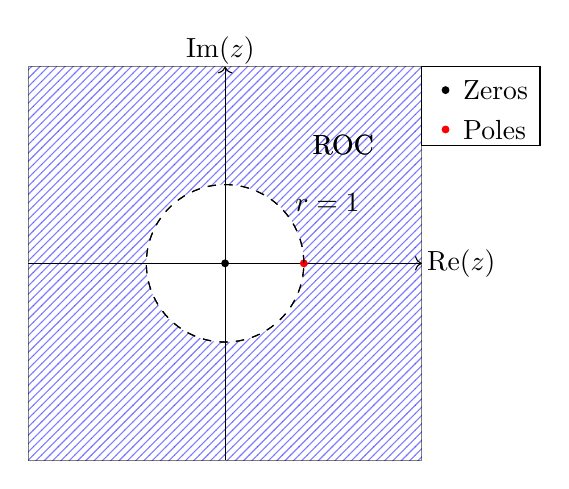
\begin{tikzpicture}
  \filldraw[pattern=north east lines, pattern color=blue, opacity=0.5] (-2.5,-2.5) rectangle (2.5,2.5);
  \fill[white] (0,0) circle [radius=1];
  \plotROC{1}{0/0}{1/0}
  % Label the ROC
  \node at (1.5,1.5) {ROC};
  % Fill the region outside the circle
\end{tikzpicture}
\end{center}
\newpage

\section{Problem 3.3 a-d}
\begin{enumerate}
\item
\[
x_1(n) = 
\begin{cases}
\wfparen{\frac{1}{3}}^{n} & \text{if } n \geq 0\\
\wfparen{\frac{1}{2}}^{-n} & \text{if } n < 0 
\end{cases}
\]
\item
\[
x_2(n) = 
\begin{cases}
\wfparen{\frac{1}{3}}^{n} - 2^{n} & \text{if } n \geq 0\\
0 & \text{if } n < 0 
\end{cases}
\]
\item $x_3(n) = x_1(n+4)$
\item $x_4(n) = x_1(-n)$
\end{enumerate}
\section{Problem 3.7}

\end{document}
  